\documentclass[a4paper,titlepage]{article}

\makeatletter
\def\input@path{{../../../template/}{./img}}
\makeatother

\usepackage{graphicx}
\usepackage[export]{adjustbox}
\usepackage{Comandi}
\usepackage{Riferimenti}
\usepackage{Stile}
\usepackage{subfiles}
\usepackage{tabularx}
\usepackage{booktabs}
\usepackage{eurosym}

\def\NOME{Analisi degli SDK dei principali assistenti virtuali}
\def\VERSIONE{1.0}
\def\DATA{2016-12-28}
\def\REDATTORE{Luca Bertolini \\ & Simeone Pizzi \\}
\def\VERIFICATORE{Andrea Magnan}
\def\RESPONSABILE{Simeone Pizzi}
\def\USO{Esterno}
\def\DESTINATARI{\COMMITTENTE \\ & \CARDIN \\ & \PROPONENTE}
\def\SOMMARIO{Documento contenente l'analisi degli SDK dei principali assistenti virtuali relativo al \gl{prodotto} \PROGETTO{} determinato dal gruppo \GRUPPO{} nel corso della realizzazione del \gl{progetto} \PROGETTO.}

\begin{document}

\maketitle

\newpage
\tableofcontents
\newpage
\listoffigures
\newpage\texttt{}
\listoftables
\newpage
\listoftables

\section{Introduzione}
	\subsection{Scopo del documento}
Questo documento riporta un analisi eseguita dal gruppo \GRUPPO{} sui principali SDK di assistenti virtuali presenti nel mercato. L'analisi in questione ha lo scopo di mettere in mostra i punti di forza e le debolezze degli SDK presi in considerazione.
	\subsection{Glossario}
	\GLOSSARIO
	\subsection{Riferimenti}
		\subsubsection{Normativi}
\begin{itemize}
\item \gl{Capitolato} d'appalto C2 - AtAVi: Accoglienza tramite Assistente Virtuale \\	\url{http://www.math.unipd.it/~tullio/IS-1/2016/Progetto/C2.pdf};
\item \NPdoc.
\end{itemize}
\section{Wit.ai}
	\subsection{Descrizione}
		\begin{minipage}{0.7\textwidth}\raggedright
			Wit.ai è una società nata nell'ottobre del 2013 e acquisita da Facebook Inc. nel 2015. \\
			L'obiettivo di Wit.ai è quello di semplificare la creazione di applicazioni che prevedono interazioni testuali o vocali; per farlo viene messa a disposizione degli sviluppatori una piattaforma di linguaggio naturale aperta ed estensibile che ha la peculiarità di apprendere tramite ogni interazione eseguita.
		\end{minipage}
		\hfill
		\noindent\begin{minipage}{0.15\textwidth}
		
\includegraphics[scale=0.6]{images/witai.jpg}
		\end{minipage}
		\subsection{Caratteristiche}
In questa sezione si vogliono elencare le principali caratteristiche del SDK in questione.
\begin{itemize}
	\item ambiente open source e totalmente gratuito per progetti sia pubblici che privati;
	\item programmatori agevolati a sviluppare grazie ai costrutti \textit{Intent} \textit{Entity}; --da spiegare cosa sono--
	\item compatibilità con molti sistemi operativi, tra cui: iOS, Android, Windows Phone, Raspberry Pi, Python e C.;
	\item \textbf{Context}: è un "object" che lo sviluppatore utilizzerà per monitorare lo stato della conversazione tra l'utente e Wit.ai. La sua principale funzione è quella di trasformare il linguaggio naturale in dati processabili da Wit;
	\item i file creati come rispos
	
\end{itemize}	
		

\section{API.ai}
	\subsection{Descrizione}
	\begin{minipage}{0.7\textwidth}\raggedright
		Api.ai è una società nata nell'ottobre del 2010 e acquisita da Google Inc. el 2016.
		API.ai è una piattaforma di conversazione che permette interazioni con il linguaggio naturale uniche nel suo genere per applicazioni, servizi e dispositivi. Gli sviluppatori possono utilizzare i servizi di riconoscimento vocale, elaborazione del linguaggio naturale e gestione della conversazione per differenziare il proprio """"buisness"""" facilmente.
	\end{minipage}
	\hfill
	\noindent\begin{minipage}{0.1\textwidth}
		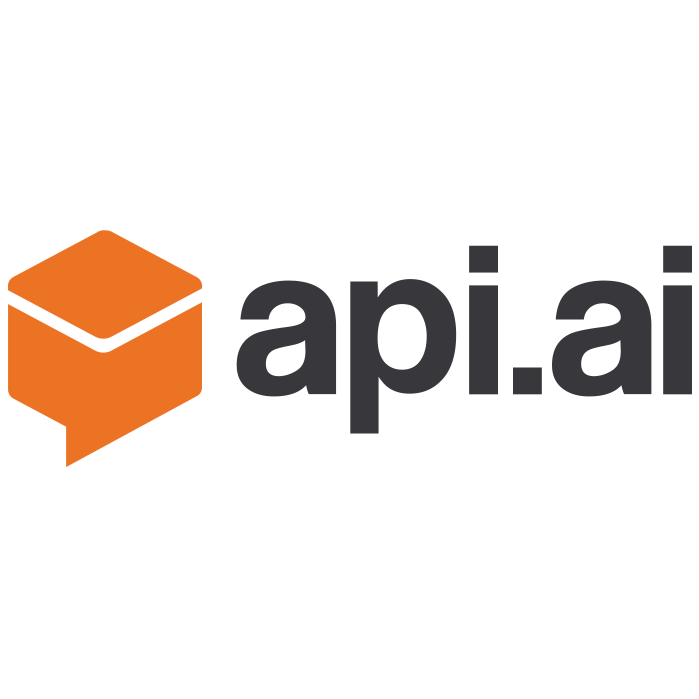
\includegraphics[scale=0.15]{images/apiai.png}
	\end{minipage}


\section{Google Assistant}
\subsection{Descrizione}

\begin{minipage}{0.7\textwidth}\raggedright
	Google Assistant è un evoluzione di Google Now, il quale risulta essere il principale assistente virtuale di Google Inc. L'assistente fornisce una comunicazione colloquiale a due vie tra l'utente e Google.
\end{minipage}
\hfill
\noindent\begin{minipage}{0.2\textwidth}
	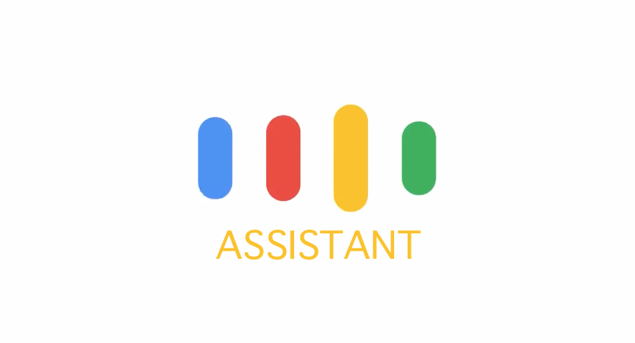
\includegraphics[scale=0.3]{images/ga.png}
\end{minipage}

\section{Siri}
\subsection{Descrizione}

\begin{minipage}{0.7\textwidth}\raggedright
	Siri nasce come applicazione indipendente per iOS resa disponibile tramite il canale commerciale App Store, per poi essere acquisita da Apple Inc. nel 2011. È presente nei dispositivi iOS, macOS, watchOS e tvOS come assistente virtuale.
\end{minipage}
\hfill
\noindent\begin{minipage}{0.1\textwidth}
	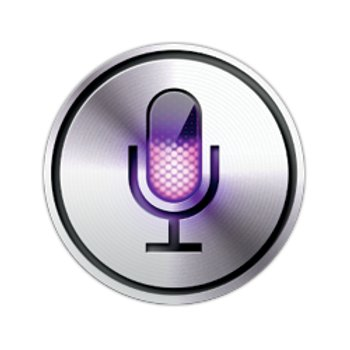
\includegraphics[scale=0.3]{images/siri.jpg}
\end{minipage}


\end{document}
